\section{Michelson-Interferometer}
\subsection{Versuchsbeschreibung}

Bei diesem Versuchsteil soll die Stabilität des Versuchsaufbaus, die Auswirkung äußerer Einflüsse sowie die Kohärenzlänge des verwendeten Lasers untersucht werden. Da uns ein neuer Versuchstisch zur Verfügung gestellt wurde, sollte auch ein Vergleich mit dem bisherigen durchgeführt werden.


\begin{figure}[ht]
 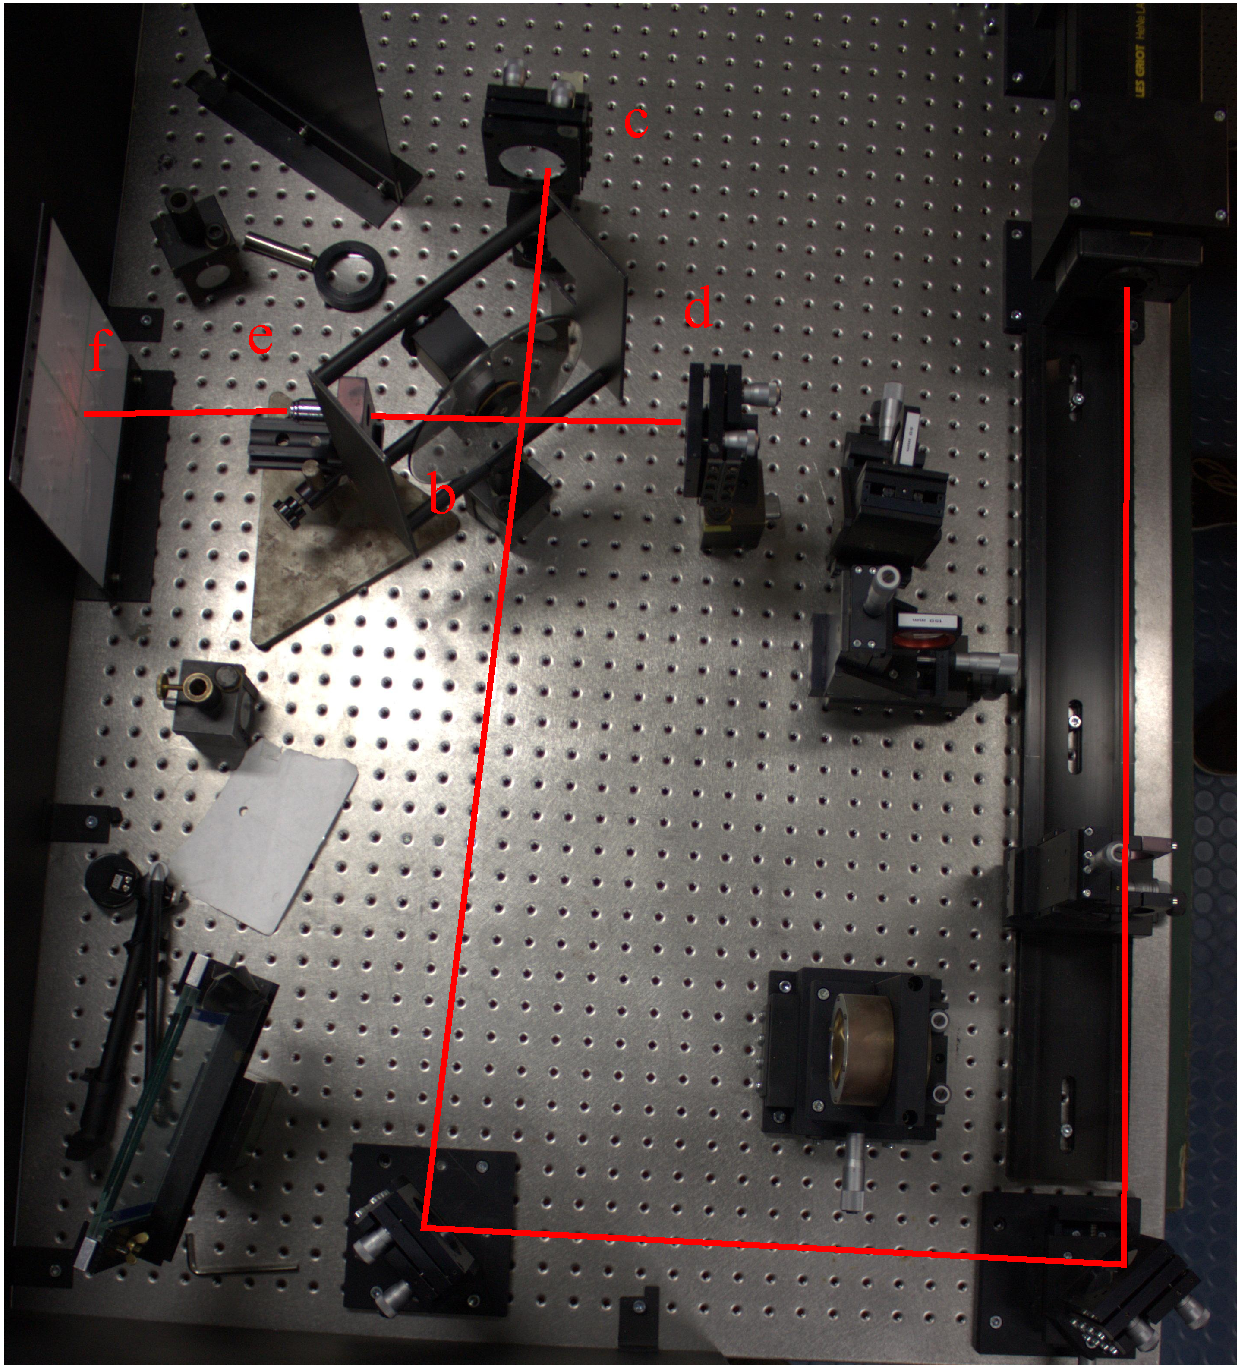
\includegraphics[width=\textwidth]{BilderAufbau/Michelson.pdf}
 \caption{Draufsicht auf das Interferometer}
 \label{aufbau_interferometer}
\end{figure}

Der Aufbau (Abb. \ref{aufbau_interferometer}) besteht aus dem Laser (a) und einem Michelson-Interferometer. Bei diesem wird am Strahlteiler (b) der Laserstrahl in zwei Komponenten geteilt. Ein Teil geht in Einfallrichtung gerade weiter und trifft auf den Spiegel (c), wo er reflektiert wird. Nachdem er zusätzlich am Strahlteiler reflektiert wurde, trifft er auf den Schirm. Der andere Teil wird bereits beim ersten Auftreffen auf den Strahlteiler reflektiert und gelangt über einen weitere Spiegel (d) ebenfalls auf den Schirm (f). Das dort beobachtete Interferenzmuster kann zusätzlich mit einem Mikroskopobjektiv (e) vergrößert werden.  

Ist der Versuchsaufbau stabil aufgebaut und sind die äußeren Störungen nicht zu groß, so sollten die Weglängen der beiden Strahlen auf dem Schirm nur orts- nicht jedoch zeitabhängig sein. Die zeitliche Stabilität des Interferenzmusters dient uns somit als Mass für die Qualität und Empfindlichkeit des Aufbaus.

Ist ein stabiles Interferenzmuster eingestellt, so kann die Kohärenzlänge des Lasers bestimmt werden. Dazu wird einer der beiden Spiegel (bei uns c) so lange verschoben bis das Interferenzmuster zusammenbricht. Der Weglängenunterschied zwischen b-d-b und b-c-b bei dem gerade noch Interferenz erkennbar ist, entspricht der Kohärenzlänge.


\subsection{Durchführung und Auswertung}

Wir haben das Michelson-Interferometer zuerst mit dem alten Tisch wie in Abb \ref{aufbau_interferometer} aufgebaut. Dabe
\begin{figure}[ht]
 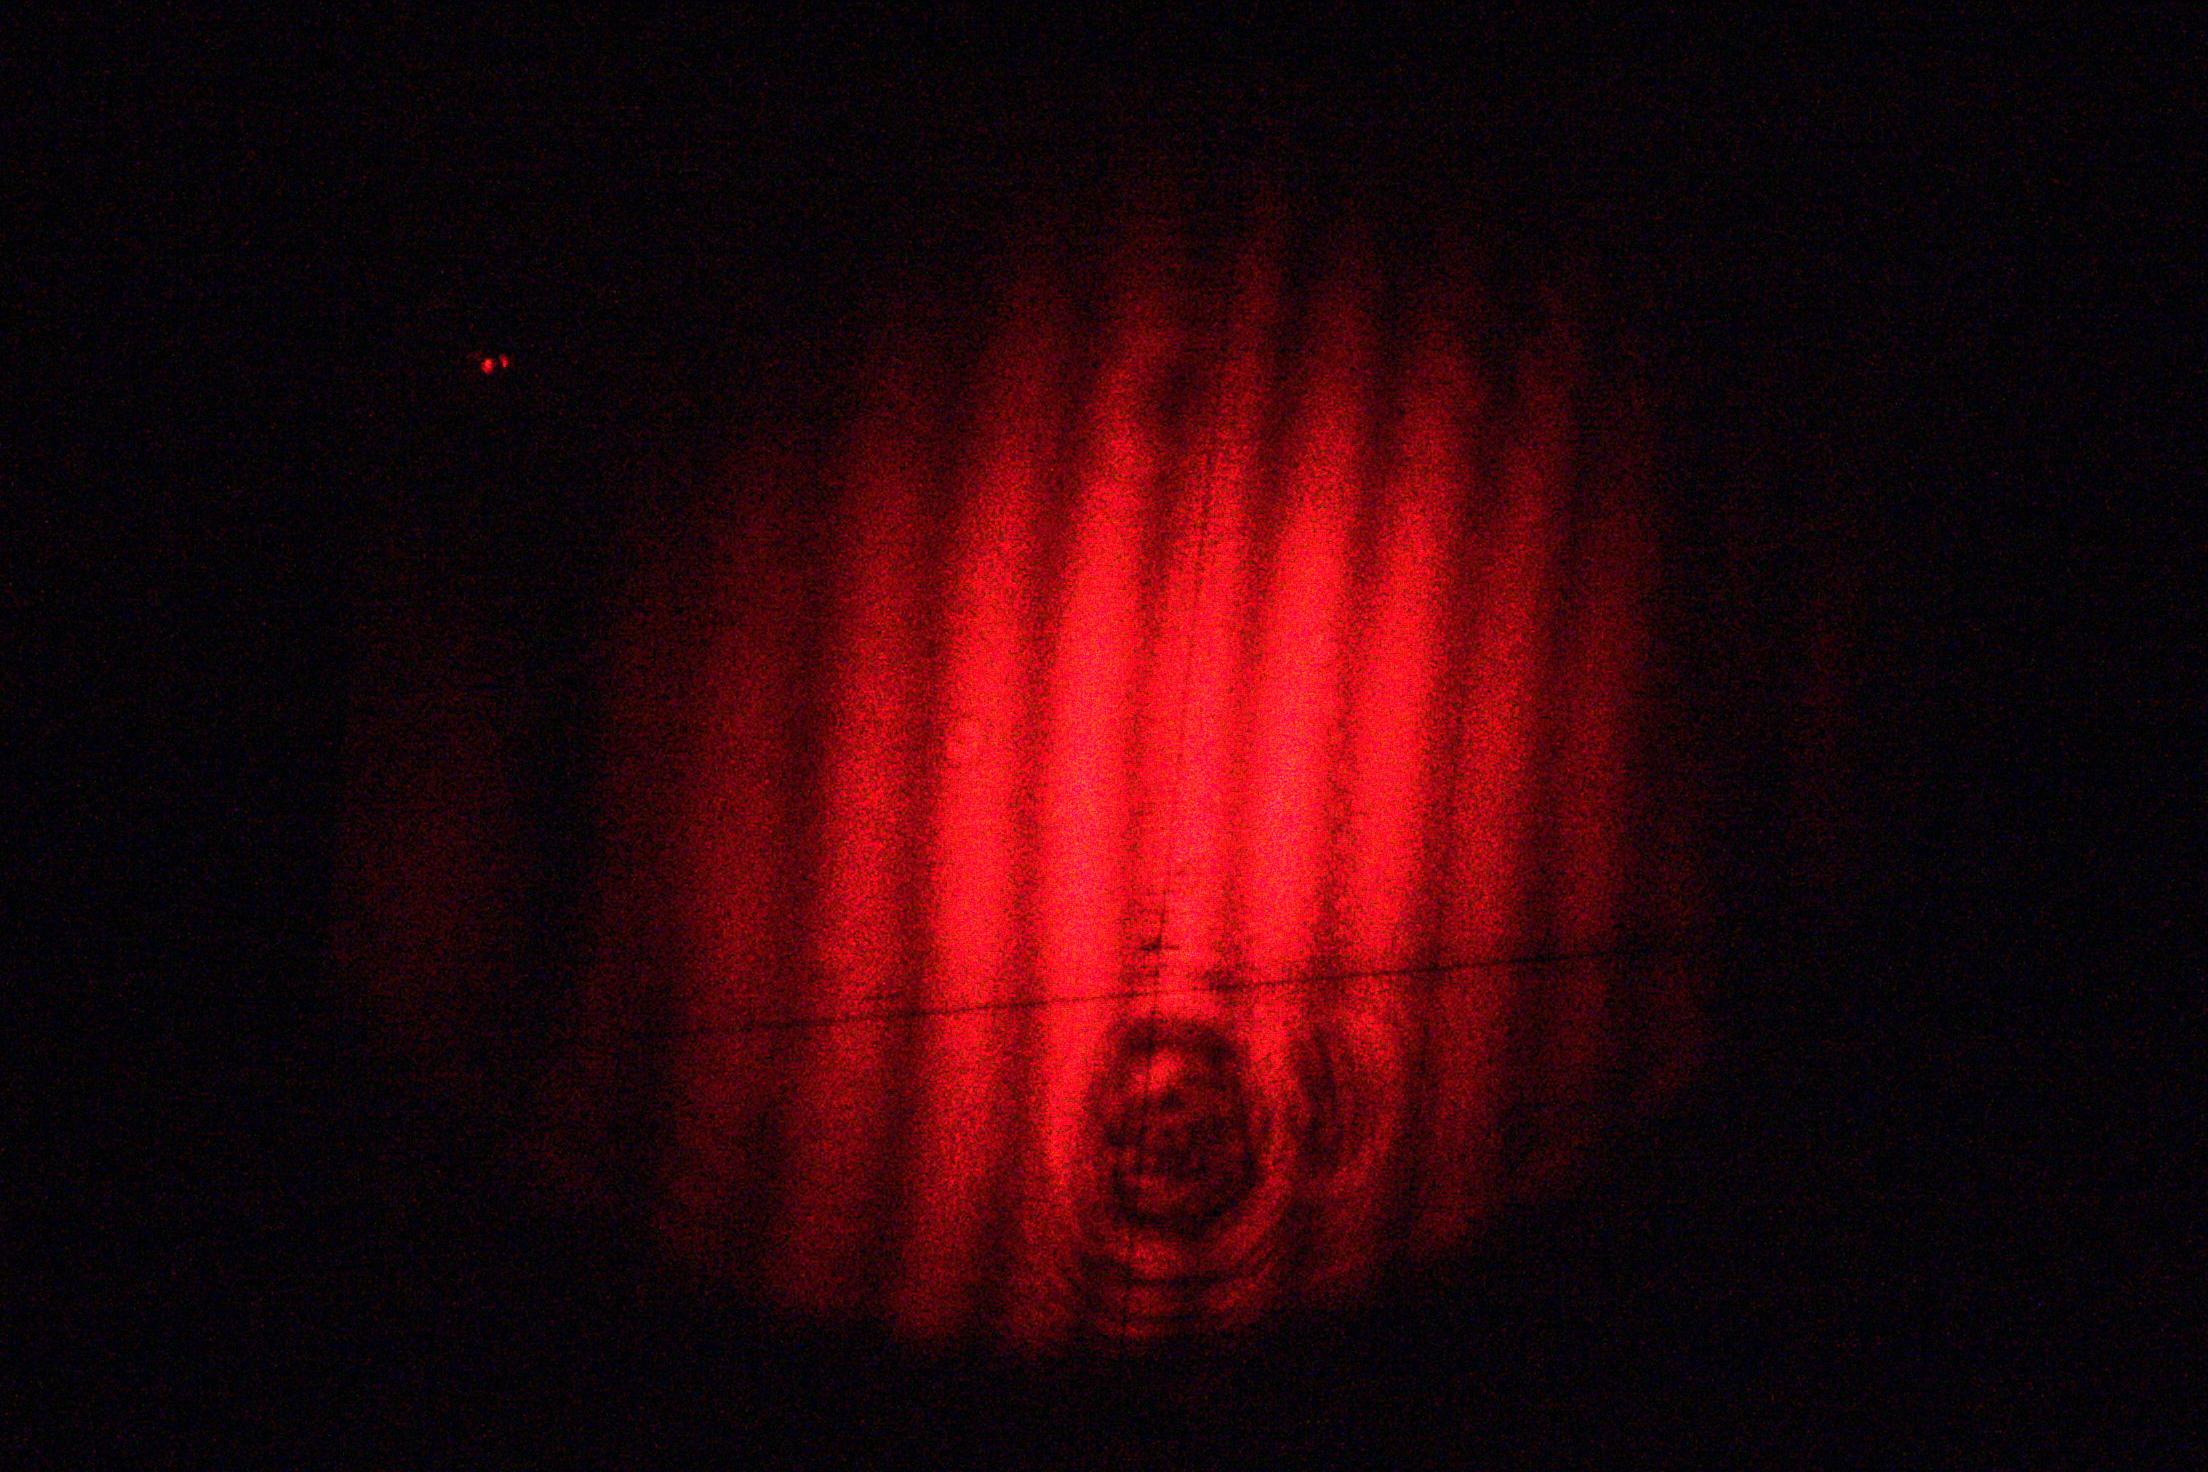
\includegraphics[width=\textwidth]{Photos/IMG_3881.jpg}
 \caption{Interferenzmuster}
\end{figure}


\begin{figure}[ht]
 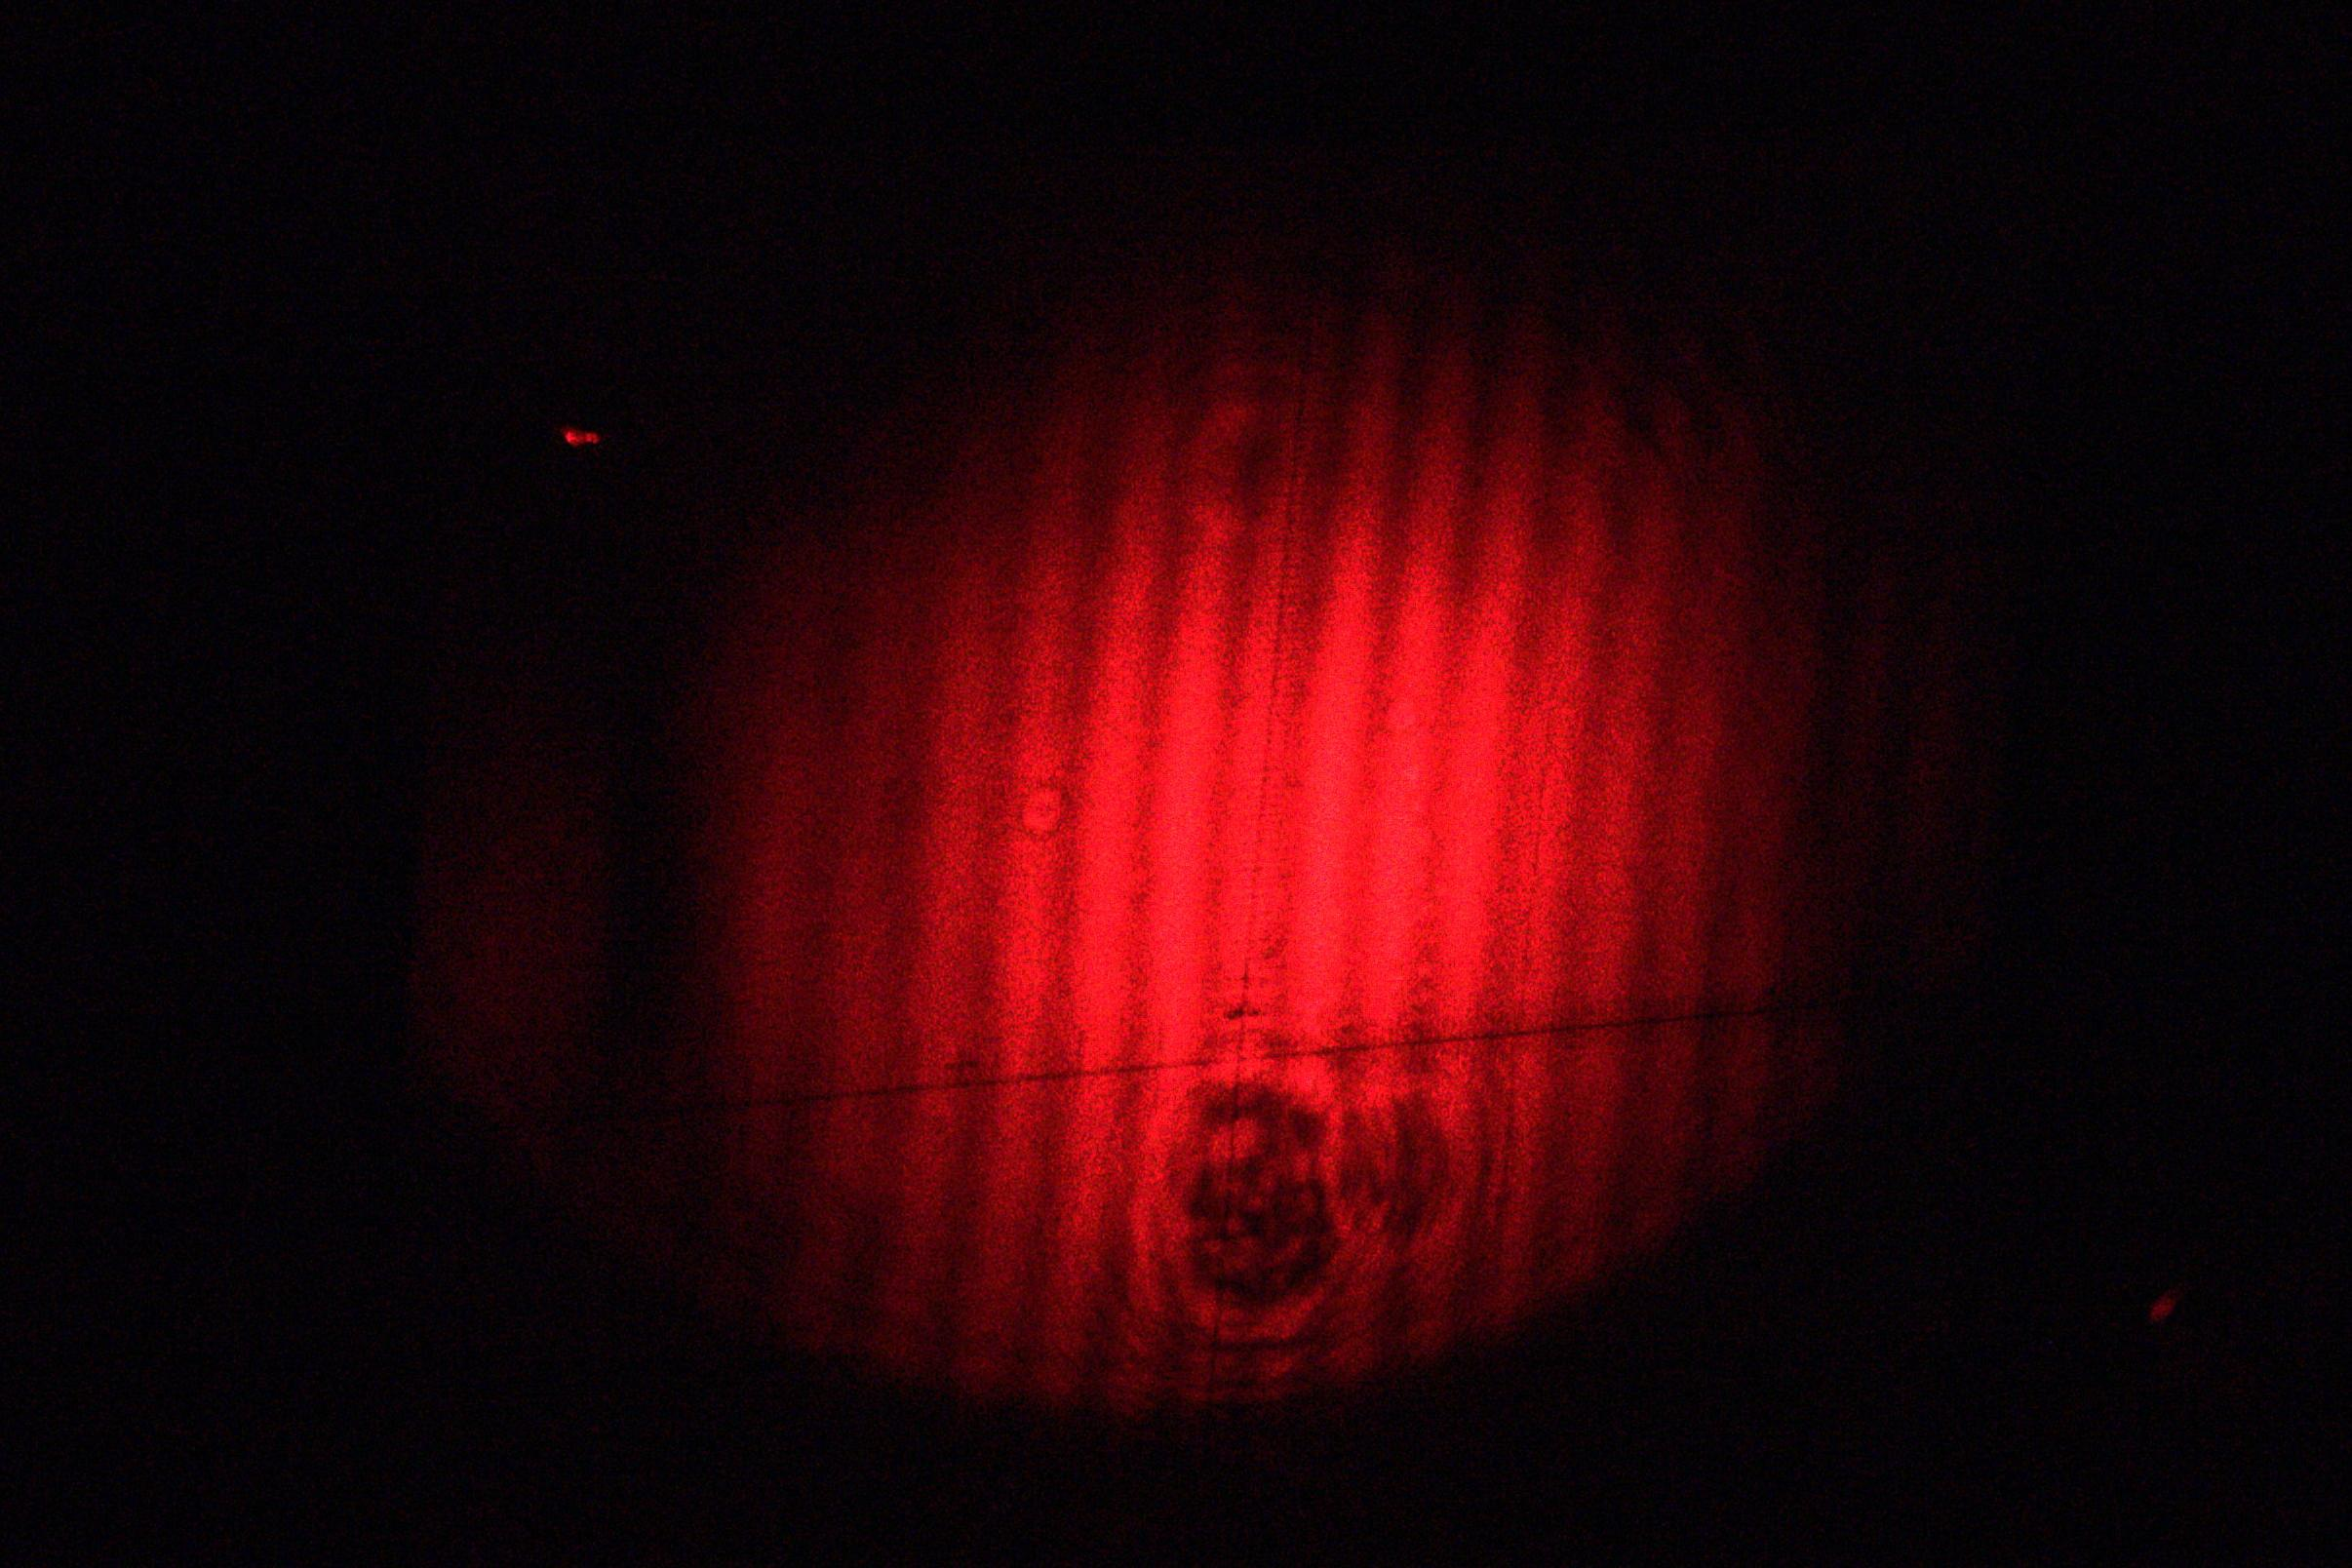
\includegraphics[width=\textwidth]{Photos/IMG_3887.jpg}
 \caption{Interferenzmuster}
\end{figure}